\PassOptionsToPackage{unicode=true}{hyperref} % options for packages loaded elsewhere
\PassOptionsToPackage{hyphens}{url}
%
\documentclass[]{article}
\usepackage{lmodern}
\usepackage{amssymb,amsmath}
\usepackage{ifxetex,ifluatex}
\usepackage{fixltx2e} % provides \textsubscript
\ifnum 0\ifxetex 1\fi\ifluatex 1\fi=0 % if pdftex
  \usepackage[T1]{fontenc}
  \usepackage[utf8]{inputenc}
  \usepackage{textcomp} % provides euro and other symbols
\else % if luatex or xelatex
  \usepackage{unicode-math}
  \defaultfontfeatures{Ligatures=TeX,Scale=MatchLowercase}
\fi
% use upquote if available, for straight quotes in verbatim environments
\IfFileExists{upquote.sty}{\usepackage{upquote}}{}
% use microtype if available
\IfFileExists{microtype.sty}{%
\usepackage[]{microtype}
\UseMicrotypeSet[protrusion]{basicmath} % disable protrusion for tt fonts
}{}
\IfFileExists{parskip.sty}{%
\usepackage{parskip}
}{% else
\setlength{\parindent}{0pt}
\setlength{\parskip}{6pt plus 2pt minus 1pt}
}
\usepackage{hyperref}
\hypersetup{
            pdftitle={Sampling Event Duration},
            pdfauthor={Alberto Dell'Era},
            pdfborder={0 0 0},
            breaklinks=true}
\urlstyle{same}  % don't use monospace font for urls
\usepackage[margin=1in]{geometry}
\usepackage{color}
\usepackage{fancyvrb}
\newcommand{\VerbBar}{|}
\newcommand{\VERB}{\Verb[commandchars=\\\{\}]}
\DefineVerbatimEnvironment{Highlighting}{Verbatim}{commandchars=\\\{\}}
% Add ',fontsize=\small' for more characters per line
\usepackage{framed}
\definecolor{shadecolor}{RGB}{248,248,248}
\newenvironment{Shaded}{\begin{snugshade}}{\end{snugshade}}
\newcommand{\AlertTok}[1]{\textcolor[rgb]{0.94,0.16,0.16}{#1}}
\newcommand{\AnnotationTok}[1]{\textcolor[rgb]{0.56,0.35,0.01}{\textbf{\textit{#1}}}}
\newcommand{\AttributeTok}[1]{\textcolor[rgb]{0.77,0.63,0.00}{#1}}
\newcommand{\BaseNTok}[1]{\textcolor[rgb]{0.00,0.00,0.81}{#1}}
\newcommand{\BuiltInTok}[1]{#1}
\newcommand{\CharTok}[1]{\textcolor[rgb]{0.31,0.60,0.02}{#1}}
\newcommand{\CommentTok}[1]{\textcolor[rgb]{0.56,0.35,0.01}{\textit{#1}}}
\newcommand{\CommentVarTok}[1]{\textcolor[rgb]{0.56,0.35,0.01}{\textbf{\textit{#1}}}}
\newcommand{\ConstantTok}[1]{\textcolor[rgb]{0.00,0.00,0.00}{#1}}
\newcommand{\ControlFlowTok}[1]{\textcolor[rgb]{0.13,0.29,0.53}{\textbf{#1}}}
\newcommand{\DataTypeTok}[1]{\textcolor[rgb]{0.13,0.29,0.53}{#1}}
\newcommand{\DecValTok}[1]{\textcolor[rgb]{0.00,0.00,0.81}{#1}}
\newcommand{\DocumentationTok}[1]{\textcolor[rgb]{0.56,0.35,0.01}{\textbf{\textit{#1}}}}
\newcommand{\ErrorTok}[1]{\textcolor[rgb]{0.64,0.00,0.00}{\textbf{#1}}}
\newcommand{\ExtensionTok}[1]{#1}
\newcommand{\FloatTok}[1]{\textcolor[rgb]{0.00,0.00,0.81}{#1}}
\newcommand{\FunctionTok}[1]{\textcolor[rgb]{0.00,0.00,0.00}{#1}}
\newcommand{\ImportTok}[1]{#1}
\newcommand{\InformationTok}[1]{\textcolor[rgb]{0.56,0.35,0.01}{\textbf{\textit{#1}}}}
\newcommand{\KeywordTok}[1]{\textcolor[rgb]{0.13,0.29,0.53}{\textbf{#1}}}
\newcommand{\NormalTok}[1]{#1}
\newcommand{\OperatorTok}[1]{\textcolor[rgb]{0.81,0.36,0.00}{\textbf{#1}}}
\newcommand{\OtherTok}[1]{\textcolor[rgb]{0.56,0.35,0.01}{#1}}
\newcommand{\PreprocessorTok}[1]{\textcolor[rgb]{0.56,0.35,0.01}{\textit{#1}}}
\newcommand{\RegionMarkerTok}[1]{#1}
\newcommand{\SpecialCharTok}[1]{\textcolor[rgb]{0.00,0.00,0.00}{#1}}
\newcommand{\SpecialStringTok}[1]{\textcolor[rgb]{0.31,0.60,0.02}{#1}}
\newcommand{\StringTok}[1]{\textcolor[rgb]{0.31,0.60,0.02}{#1}}
\newcommand{\VariableTok}[1]{\textcolor[rgb]{0.00,0.00,0.00}{#1}}
\newcommand{\VerbatimStringTok}[1]{\textcolor[rgb]{0.31,0.60,0.02}{#1}}
\newcommand{\WarningTok}[1]{\textcolor[rgb]{0.56,0.35,0.01}{\textbf{\textit{#1}}}}
\usepackage{graphicx,grffile}
\makeatletter
\def\maxwidth{\ifdim\Gin@nat@width>\linewidth\linewidth\else\Gin@nat@width\fi}
\def\maxheight{\ifdim\Gin@nat@height>\textheight\textheight\else\Gin@nat@height\fi}
\makeatother
% Scale images if necessary, so that they will not overflow the page
% margins by default, and it is still possible to overwrite the defaults
% using explicit options in \includegraphics[width, height, ...]{}
\setkeys{Gin}{width=\maxwidth,height=\maxheight,keepaspectratio}
\setlength{\emergencystretch}{3em}  % prevent overfull lines
\providecommand{\tightlist}{%
  \setlength{\itemsep}{0pt}\setlength{\parskip}{0pt}}
\setcounter{secnumdepth}{0}
% Redefines (sub)paragraphs to behave more like sections
\ifx\paragraph\undefined\else
\let\oldparagraph\paragraph
\renewcommand{\paragraph}[1]{\oldparagraph{#1}\mbox{}}
\fi
\ifx\subparagraph\undefined\else
\let\oldsubparagraph\subparagraph
\renewcommand{\subparagraph}[1]{\oldsubparagraph{#1}\mbox{}}
\fi

% set default figure placement to htbp
\makeatletter
\def\fps@figure{htbp}
\makeatother


\title{Sampling Event Duration}
\author{Alberto Dell'Era}
\date{}

\begin{document}
\maketitle

\emph{A short summary is available at:
\url{https://github.com/alberto-dellera/sampling_event_duration/blob/master/README.md}}

\emph{Github readers: github on-line resolution is very low, and the pdf
can be even truncated(!)\\
I'd suggest to download this pdf and open it locally}

\hypertarget{abstract}{%
\section{Abstract}\label{abstract}}

We will study an event sampling process whose sampling period is
uniform:

\begin{center}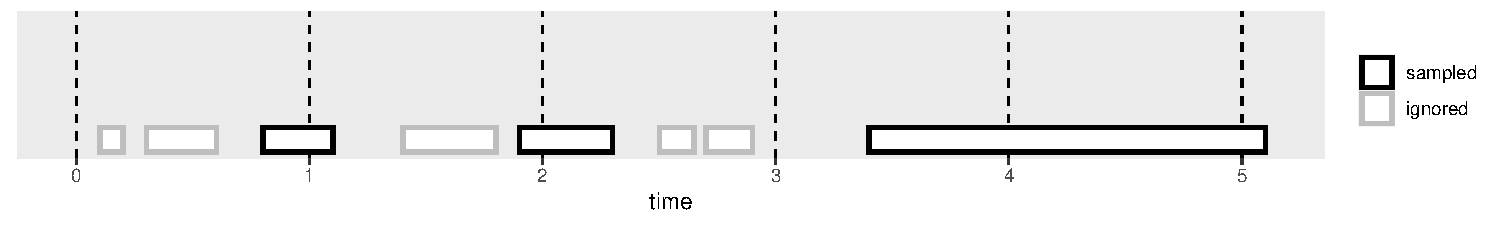
\includegraphics[width=1.0\textwidth]{sampling_event_duration_files/figure-latex/abstract_sampling_illustration-1} \end{center}

The process samples the duration of the events that are active
(``in-flight'') at sample time, and ignores all the others.

We will derive the probability distribution of the sampled durations
given the original durations distribution in general, but focusing on
the versatile Gamma distribution. We will build random generators to
simulate the sampling process, and then design a Bayesian estimator to
infer back the original distribution parameters, implemented in Stan.

\hypertarget{introduction}{%
\section{Introduction}\label{introduction}}

Consider performing a marketing survey to study the behaviour of
customers of a huge physical library (or maybe an on-line retailer). To
reduce the study cost, a plausible policy might be to visit the library
every hour and interview every one inside, ignoring other customers that
enter the library later on the same hour.

Imagine that one of the dimensions logged is ``time spent inside the
library''. Since we will sample every one that spends more than one hour
inside, but only half of people spending half an hour, one sixth of
customers spending ten minutes, and so on, the sampled data will not be
an accurate representation of the actual distribution of the
inside-library duration. We would, for example, sadly overestimate the
book-lovers proportion.

But if we know the theoretical distribution of the original data, we can
in principle estimate its parameters from the samples, and obtain a
cleanest picture.

A real-life example of such a sampling process can be found in IT.
Specialists in software performance optimization make extensive use of
\emph{statistical profilers}\footnote{\url{https://en.wikipedia.org/wiki/Profiling_(computer_programming)\#Statistical_profilers}}:
tools that sample running programs execution at regular intervals and
register what they were doing (e.g.~waiting for disk, running on the
CPU) for later analysis. These tools usually register only the
occurrence on an event, not its duration; a notable exception is
Oracle©® ASH\footnote{this is actually the tool that sparked my interest
  for this statistical problem. I've been using it for years, when
  dressing the hat of Oracle Performance Tuning specialist, one of my
  preferred outfits.}, that samples the duration as well. Check
(Beresniewicz \protect\hyperlink{ref-ASHMATH}{2020}), especially slide
33, for an extensive discussion.

This paper is my personal journey into this fascinating inference
problem, limited to simulated data for simplicity and lack of time, that
might be a good starting point for someone interested in inferring from
real data.

It's a Bayesian journey out of personal preference, but a Frequentist
might easily adapt most of the paper for her toolbox; for example, an
extension to MLE should be very simple, as hinted in the discussion.

Last but not least: everything is demonstrated using a reproducible R
Markdown document, and I have strived to write the cleanest code
possible and to carefully document it.

\hypertarget{probability-distribution-of-the-samples}{%
\section{Probability Distribution of the
samples}\label{probability-distribution-of-the-samples}}

Letting \(x \sim f(x)\) the event duration random variable and
\(y \sim g(y)\) the sampled one, we can easily derive the latter from
the former by observing that the probability that \(x\) is sampled is
proportional to \(x/T\) for \(x<T\) (e.g.~if \(x\) is half as long as
\(T\), its sampling probability is 0.5) and is 1 for \(x>=T\). Hence we
just need to multiply \(f(x)\) by the hinge function \[ h(x) \triangleq
    \begin{cases}
      x/T & x < T \\
      1 & x >= T
    \end{cases}
\] and then renormalize, obtaining \[
g(y) = p(y=x) =  \frac{h(x)f(x)}{\eta}\ ;\ \ \ \ \ \  \eta \triangleq \int_{0}^{\infty} h(\tau)f(\tau) d\tau
\] We can further decompose \(\eta\) as \(\eta = \eta_A + \eta_B\),
where \[
 \eta_A \triangleq \int_{0}^{T} h(\tau)f(\tau) d\tau = \frac{1}{T} \int_{0}^{T} \tau f(\tau) d\tau
 \]

\[\eta_B \triangleq \int_{T}^{\infty} h(\tau)f(\tau) d\tau = \int_{T}^{\infty} f(\tau) d\tau = 1 - \int_{0}^{T} f(\tau) d\tau = 1 - F(T)
\] Note that \(\eta_A\) is essentially the average value of \(x\) over
the interval \([0,T)\), and \(\eta_B\) is based on the CDF of the
distribution; if \(f(x)\) is a well-known distribution, both are usually
readily available, at least numerically approximated.

\hypertarget{focus-on-the-gamma-distribution}{%
\subsection{Focus on the Gamma
Distribution}\label{focus-on-the-gamma-distribution}}

Let's now focus on the case of the Gamma distribution, very important in
the context of durations\footnote{mostly because of its versatility: it
  includes the important exponential as a special case, and can
  approximate the normal itself well for high values of \emph{shape}}.

\[
  f(x) = Gamma(x | \alpha,\beta) = \frac{\beta^\alpha}{\Gamma(\alpha)} x^{\alpha-1}e^{-\beta x} 
\] where \(\alpha\) is usually named the ``shape'' and \(\beta\) the
``rate''.

For \(x<T\) we have of course \[
  g(y) = p(y=x) = \frac{x}{T} * Gamma(x | \alpha,\beta) \frac{1}{\eta}
\] But, algebraically: \[
  x * Gamma(x | \alpha,\beta) = 
  \frac{\beta^\alpha}{\Gamma(\alpha)} x^{(\alpha+1)-1}e^{-\beta x} = 
  \beta^{-1} \frac{\Gamma(\alpha+1)}{\Gamma(\alpha)}Gamma(x|\alpha+1,\beta) \ \ \ (1)
\] that is \[
 x \sim Gamma(\alpha, \beta)   \implies y \sim (const) * Gamma(\alpha+1, \beta); \ \ \ for \ x < T 
\]

hence the \emph{effect of sampling is simply to increase the shape by
1}, normalization constants apart. Amazing\footnote{if developed
  further, this result could probably give some insights about the
  physical meaning of ``shape''.} !

A practical benefit of (1) is that we can easily write \(\eta\), the
most difficult part of the density expression, as a function of Gamma
(FGamma being the CDF): \[
  \eta_A = \frac{1}{T} \beta^{-1} \frac{\Gamma(\alpha+1)}{\Gamma(\alpha)}FGamma(T|\alpha+1,\beta);\ \ \  \eta_B = 1 - FGamma(T|\alpha,\beta)
\] In R, that becomes:

\begin{Shaded}
\begin{Highlighting}[]
\CommentTok{#' Density of the Sampled Gamma Distribution}
\CommentTok{#'}
\CommentTok{#' @param x     Vector of random variable values}
\CommentTok{#' @param shape The original Gamma "shape" parameter}
\CommentTok{#' @param rate  The original Gamma "rate" parameter}
\CommentTok{#' @param T     The sampling period}
\CommentTok{#' @param log   If TRUE, returns the log density}
\CommentTok{#'}
\CommentTok{#' @return Vector of (log) densities}
\NormalTok{dsgamma <-}\StringTok{ }\ControlFlowTok{function}\NormalTok{(x, shape, rate, T, }\DataTypeTok{log=}\OtherTok{FALSE}\NormalTok{) \{}
\NormalTok{  T.log <-}\StringTok{ }\NormalTok{base}\OperatorTok{::}\KeywordTok{log}\NormalTok{(T)}
  
  \CommentTok{# calc eta}
\NormalTok{  A.log <-}\StringTok{ }\NormalTok{(}\OperatorTok{-}\NormalTok{T.log) }\OperatorTok{+}\StringTok{ }
\StringTok{           }\NormalTok{(}\OperatorTok{-}\NormalTok{base}\OperatorTok{::}\KeywordTok{log}\NormalTok{(rate)) }\OperatorTok{+}\StringTok{ }
\StringTok{           }\KeywordTok{lgamma}\NormalTok{(shape}\OperatorTok{+}\DecValTok{1}\NormalTok{) }\OperatorTok{-}\StringTok{ }\KeywordTok{lgamma}\NormalTok{(shape) }\OperatorTok{+}\StringTok{ }\KeywordTok{pgamma}\NormalTok{(T, }\DataTypeTok{shape=}\NormalTok{shape}\OperatorTok{+}\DecValTok{1}\NormalTok{, }\DataTypeTok{rate=}\NormalTok{rate, }\DataTypeTok{log.p=}\OtherTok{TRUE}\NormalTok{) }
\NormalTok{  A <-}\StringTok{ }\KeywordTok{exp}\NormalTok{(A.log)}
\NormalTok{  B <-}\StringTok{ }\FloatTok{1.0} \OperatorTok{-}\StringTok{ }\KeywordTok{pgamma}\NormalTok{(T, }\DataTypeTok{shape=}\NormalTok{shape, }\DataTypeTok{rate=}\NormalTok{rate) }
\NormalTok{  eta.log <-}\StringTok{ }\KeywordTok{log}\NormalTok{(A }\OperatorTok{+}\StringTok{ }\NormalTok{B)}
  
  \CommentTok{# calc density}
\NormalTok{  x  <-}\StringTok{ }\KeywordTok{ifelse}\NormalTok{(x }\OperatorTok{>}\StringTok{ }\NormalTok{.Machine}\OperatorTok{$}\NormalTok{double.eps, x, }\OtherTok{NA}\NormalTok{)}
\NormalTok{  f.log <-}\StringTok{ }\KeywordTok{dgamma}\NormalTok{(x, }\DataTypeTok{shape=}\NormalTok{shape, }\DataTypeTok{rate=}\NormalTok{rate, }\DataTypeTok{log=}\OtherTok{TRUE}\NormalTok{)}
\NormalTok{  h.log <-}\StringTok{ }\KeywordTok{ifelse}\NormalTok{(x }\OperatorTok{<}\StringTok{ }\NormalTok{T, base}\OperatorTok{::}\KeywordTok{log}\NormalTok{(x) }\OperatorTok{-}\StringTok{ }\NormalTok{T.log, }\FloatTok{0.0}\NormalTok{)}
\NormalTok{  g.log <-}\StringTok{ }\KeywordTok{ifelse}\NormalTok{(}\KeywordTok{is.na}\NormalTok{(x), }\OperatorTok{-}\OtherTok{Inf}\NormalTok{, f.log }\OperatorTok{+}\StringTok{ }\NormalTok{h.log }\OperatorTok{-}\StringTok{ }\NormalTok{eta.log)}
  \ControlFlowTok{if}\NormalTok{ (log) \{}
    \KeywordTok{return}\NormalTok{ (g.log)}
\NormalTok{  \}}
  \KeywordTok{exp}\NormalTok{(g.log)}
\NormalTok{\}}
\end{Highlighting}
\end{Shaded}

\hypertarget{discussion}{%
\subsection{discussion}\label{discussion}}

Let's plot the densities for a few interesting cases:

\begin{center}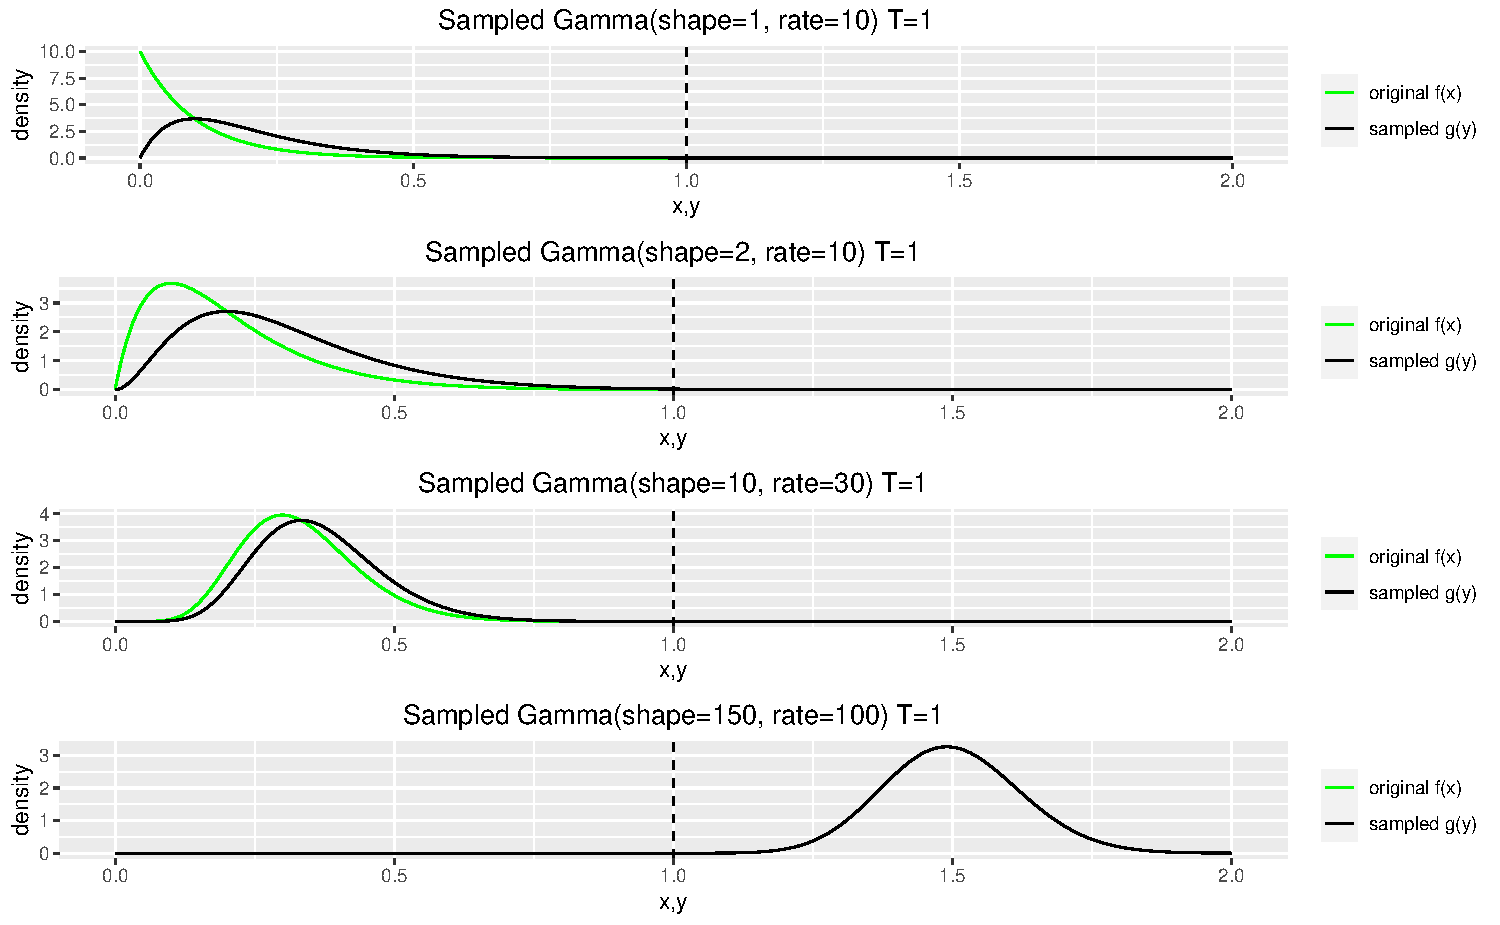
\includegraphics[width=1.0\textwidth]{sampling_event_duration_files/figure-latex/dsgamma_discussion-1} \end{center}

The first plot is the case of the ubiquitous exponential distribution.
The sampling distortion is quite dramatic: the exponential silhouette is
gone; small durations, that used to concentrate most of the mass, have
almost disappeared, and the mode itself has shifted from zero to about
0.1.

In the second case, the distortion is still quite noticeable; only in
the third case, when the shape has got to 10, the distortion is
relatively minimal.

The fourth plot shows the case of a distribution whose mass is well
above the sampling period. As expected, the sampled distribution is
virtually the same as the original.

\hypertarget{random-generators-and-simulation}{%
\section{Random Generators and
Simulation}\label{random-generators-and-simulation}}

We now discuss two numerical methods for drawing random numbers from the
sampled distribution \(g(x)\) given a drawing function for \(f(x)\), a
crucial task for any serious application.

\hypertarget{by-physical-process-simulation}{%
\subsection{by physical process
simulation}\label{by-physical-process-simulation}}

The most straightforward way is to directly implement the physical
sampling process:

\begin{Shaded}
\begin{Highlighting}[]
\CommentTok{#' Draw samples y distributed as g(y) from the original distribution f(x), }
\CommentTok{#'   by simulating the physical process}
\CommentTok{#'}
\CommentTok{#' @param n      The number of draws desired from g(y) (i.e. length of y)}
\CommentTok{#' @param f      A function that draws n numbers from the original durations distribution}
\CommentTok{#' @param T      The sampling period}
\CommentTok{#' @param b      A function that draws n numbers from the distribution of in-between time}
\CommentTok{#' @param fill.x Whether to return the original x draws}
\CommentTok{#'}
\CommentTok{#' @return a list of two vectors: "x" with all the draws, and "y" for the sampled subset}
\NormalTok{rsampled.phy <-}\StringTok{ }\ControlFlowTok{function}\NormalTok{(n, f, T, }\DataTypeTok{b=}\OtherTok{NULL}\NormalTok{, }\DataTypeTok{fill.x=}\OtherTok{FALSE}\NormalTok{) \{}
\NormalTok{  y <-}\StringTok{ }\KeywordTok{rep}\NormalTok{(}\OperatorTok{-}\DecValTok{1}\NormalTok{, n)}
\NormalTok{  x <-}\StringTok{ }\KeywordTok{numeric}\NormalTok{(}\DecValTok{0}\NormalTok{)}
\NormalTok{  xi <-}\StringTok{ }\DecValTok{0}\NormalTok{; yi <-}\StringTok{ }\DecValTok{0}
\NormalTok{  sta <-}\StringTok{ }\DecValTok{0}\NormalTok{; sto <-}\StringTok{ }\OtherTok{NA}
  
  \ControlFlowTok{repeat}\NormalTok{ \{}
    \CommentTok{# draw x from f(x)}
\NormalTok{    dur <-}\StringTok{ }\KeywordTok{f}\NormalTok{(}\DecValTok{1}\NormalTok{)}
    \ControlFlowTok{if}\NormalTok{ (dur }\OperatorTok{<}\StringTok{ }\DecValTok{0}\NormalTok{) }\KeywordTok{stop}\NormalTok{(}\KeywordTok{paste0}\NormalTok{(}\StringTok{"negative duration from f: "}\NormalTok{, dur))}
\NormalTok{    sto <-}\StringTok{ }\NormalTok{sta }\OperatorTok{+}\StringTok{ }\NormalTok{dur}
    
    \CommentTok{# store x if so desired}
    \ControlFlowTok{if}\NormalTok{ (fill.x) \{}
\NormalTok{      xi <-}\StringTok{ }\NormalTok{xi }\OperatorTok{+}\StringTok{ }\DecValTok{1}
      \ControlFlowTok{if}\NormalTok{ (xi }\OperatorTok{>}\StringTok{ }\KeywordTok{length}\NormalTok{(x)) \{}
\NormalTok{        x <-}\StringTok{ }\KeywordTok{append}\NormalTok{(x, }\KeywordTok{rep}\NormalTok{(}\OtherTok{NA}\NormalTok{, }\DecValTok{10}\OperatorTok{*}\NormalTok{n))}
\NormalTok{      \}  }
\NormalTok{      x[xi] <-}\StringTok{ }\NormalTok{dur}
\NormalTok{    \}}
     
    \CommentTok{# sample x as y if across sampling instant }
    \ControlFlowTok{if}\NormalTok{ (}\KeywordTok{floor}\NormalTok{(sta}\OperatorTok{/}\NormalTok{T) }\OperatorTok{<}\StringTok{ }\KeywordTok{floor}\NormalTok{(sto}\OperatorTok{/}\NormalTok{T)) \{}
\NormalTok{      yi <-}\StringTok{ }\NormalTok{yi }\OperatorTok{+}\StringTok{ }\DecValTok{1}
\NormalTok{      y[yi] <-}\StringTok{ }\NormalTok{dur}
      \ControlFlowTok{if}\NormalTok{ (yi }\OperatorTok{==}\StringTok{ }\NormalTok{n) }\ControlFlowTok{break}
\NormalTok{    \}}
    
    \CommentTok{# draw from the in-between distribution}
    \ControlFlowTok{if}\NormalTok{ (}\OperatorTok{!}\KeywordTok{is.null}\NormalTok{(b)) \{}
\NormalTok{      dur_break <-}\StringTok{ }\KeywordTok{b}\NormalTok{(}\DecValTok{1}\NormalTok{)}
      \ControlFlowTok{if}\NormalTok{ (dur_break }\OperatorTok{<}\StringTok{ }\DecValTok{0}\NormalTok{) }\KeywordTok{stop}\NormalTok{(}\KeywordTok{paste0}\NormalTok{(}\StringTok{"negative duration from b: "}\NormalTok{, dur_break))}
\NormalTok{      sto <-}\StringTok{ }\NormalTok{sto }\OperatorTok{+}\StringTok{ }\NormalTok{dur_break}
\NormalTok{    \}}
    
\NormalTok{    sta <-}\StringTok{ }\NormalTok{sto}
\NormalTok{  \}}
  \KeywordTok{list}\NormalTok{(}\DataTypeTok{x=}\NormalTok{x[}\DecValTok{1}\OperatorTok{:}\NormalTok{xi], }\DataTypeTok{y=}\NormalTok{y)}
\NormalTok{\}}
\end{Highlighting}
\end{Shaded}

This trivial function simply draws a duration from the provided
\(f(x)\), sets accordingly the start and stop extremata of the event,
and if the interval crosses the sampling instant it returns the duration
as \(y\). It can optionally store all the original draws from \(x\)
(which the \(y\) vector is a subset of).

Side note: to accurately simulate the physical process, an optional
\(b(x)\) distribution can be provided to model the time in-between
events. This distribution does not alter\footnote{this is because the
  \emph{stopping intention} of this function is to stop when \(n\)
  samples have been provided. If the stopping intention were, say, to
  stop after a certain time has elapsed, the number of samples would be
  a random variable, not a given number, influenced by \(b(x)\) as well
  as \(f(x)\). This is actually the most common real-life scenario but
  it is considerably more complex to handle and hence out-of-scope for
  this paper, that focuses on the fundamental theory; for the
  intricacies of this sampling intention see (Kruschke
  \protect\hyperlink{ref-DBDA2E}{2015}, 308, ``With intention to fix
  duration''), in the context of p-values. Anecdotally, the stopping
  intention should not change the results that much for practical
  applications.} the density of the returned \(y\) random variate, but
it could change the average size of \(x\) (for example, if
\(f(x) \equiv b(x)\), the expected size of \(x\) would be twice as
long). \(b(x)\) will never be used in this paper, but can be useful for
other purposes.

A call example is the specialization for the Gamma distribution that we
will use from now on:

\begin{Shaded}
\begin{Highlighting}[]
\NormalTok{rsgamma.phy <-}\StringTok{ }\ControlFlowTok{function}\NormalTok{(n, shape, rate, T, }\DataTypeTok{b=}\OtherTok{NULL}\NormalTok{, }\DataTypeTok{fill.x=}\OtherTok{FALSE}\NormalTok{) \{}
\NormalTok{  f <-}\StringTok{ }\ControlFlowTok{function}\NormalTok{(n) \{}
    \KeywordTok{rgamma}\NormalTok{(n, }\DataTypeTok{shape=}\NormalTok{shape, }\DataTypeTok{rate=}\NormalTok{rate)}
\NormalTok{  \}}
  \KeywordTok{rsampled.phy}\NormalTok{(n, f, T, b, fill.x)}
\NormalTok{\}}

\KeywordTok{set.seed}\NormalTok{(}\DecValTok{5}\NormalTok{)}
\KeywordTok{rsgamma.phy}\NormalTok{(}\DecValTok{2}\NormalTok{, }\DataTypeTok{shape=}\DecValTok{1}\NormalTok{, }\DataTypeTok{rate=}\DecValTok{1}\NormalTok{, }\DataTypeTok{T=}\FloatTok{1.0}\NormalTok{, }\DataTypeTok{fill.x=}\OtherTok{TRUE}\NormalTok{)}
\end{Highlighting}
\end{Shaded}

\begin{verbatim}
## $x
## [1] 0.08218487 0.17824958 0.55082843 2.44242891 0.16455419 0.61080940
## 
## $y
## [1] 2.4424289 0.6108094
\end{verbatim}

\hypertarget{by-rejection-sampling}{%
\subsection{by rejection sampling}\label{by-rejection-sampling}}

Another possibility is to draw a duration, and then accept it as a
sample with probability \(h(x)\):

\begin{Shaded}
\begin{Highlighting}[]
\CommentTok{#' Draw samples y distributed as g(y) from the original distribution f(x), }
\CommentTok{#'   by acceptance/rejection sampling accordingly to h(x)}
\CommentTok{#'}
\CommentTok{#' @param n      The number of draws desired from g(y) (i.e. length of y)}
\CommentTok{#' @param f      A function that draws n numbers from the original durations distribution}
\CommentTok{#' @param T      The sampling period}
\CommentTok{#'}
\CommentTok{#' @return a vector containing the sampled y}
\NormalTok{rsampled.rej <-}\StringTok{ }\ControlFlowTok{function}\NormalTok{(n, f, T) \{}
\NormalTok{  y <-}\StringTok{ }\KeywordTok{rep}\NormalTok{(}\OperatorTok{-}\DecValTok{1}\NormalTok{, n)}
\NormalTok{  yi <-}\StringTok{ }\DecValTok{0}
  \ControlFlowTok{repeat}\NormalTok{ \{}
\NormalTok{    dur <-}\StringTok{ }\KeywordTok{f}\NormalTok{(}\DecValTok{1}\NormalTok{)}
    \ControlFlowTok{if}\NormalTok{ (dur }\OperatorTok{<}\StringTok{ }\DecValTok{0}\NormalTok{) }\KeywordTok{stop}\NormalTok{(}\KeywordTok{paste0}\NormalTok{(}\StringTok{"negative duration from f: "}\NormalTok{, dur))}
\NormalTok{    h =}\StringTok{ }\KeywordTok{ifelse}\NormalTok{(dur }\OperatorTok{<}\StringTok{ }\NormalTok{T, dur}\OperatorTok{/}\NormalTok{T, }\DecValTok{1}\NormalTok{)}
\NormalTok{    p <-}\StringTok{ }\KeywordTok{runif}\NormalTok{(}\DecValTok{1}\NormalTok{)}
    \ControlFlowTok{if}\NormalTok{ (h }\OperatorTok{>}\StringTok{ }\NormalTok{p) \{}
      \CommentTok{# accept}
\NormalTok{      yi <-}\StringTok{ }\NormalTok{yi }\OperatorTok{+}\StringTok{ }\DecValTok{1}
\NormalTok{      y[yi] <-}\StringTok{ }\NormalTok{dur}
      \ControlFlowTok{if}\NormalTok{ (yi }\OperatorTok{==}\StringTok{ }\NormalTok{n) }\ControlFlowTok{break}
\NormalTok{    \} }\ControlFlowTok{else}\NormalTok{ \{}
      \CommentTok{#reject}
\NormalTok{    \}}
\NormalTok{  \}}
\NormalTok{  y}
\NormalTok{\}}
\end{Highlighting}
\end{Shaded}

This is a great example of the classic technique of
\href{https://en.wikipedia.org/wiki/Rejection_sampling}{acceptance-rejection
sampling}. Actually, it is a marvelous example of an
acceptance-rejection sampling that \emph{happens physically}, not as a
numeric artifact to efficiently draw random numbers from distributions.

The drawback of rsampled.rej (and rsampled.phy actually) is that it is
slow for distributions whose mass is concentrated near very small
values; for example, for durations around 1e-3 it takes 1000 draws for
each \(y\) on average. Speed is anyway adequate for our
purposes\footnote{I was experimenting with faster alternatives when time
  ran out; I might pursue that road again in the future.}.

Call example, and specialization for the Gamma distribution:

\begin{Shaded}
\begin{Highlighting}[]
\NormalTok{rsgamma.rej <-}\StringTok{ }\ControlFlowTok{function}\NormalTok{(n, shape, rate, T) \{}
\NormalTok{  f <-}\StringTok{ }\ControlFlowTok{function}\NormalTok{(n) \{}
    \KeywordTok{rgamma}\NormalTok{(n, }\DataTypeTok{shape=}\NormalTok{shape, }\DataTypeTok{rate=}\NormalTok{rate)}
\NormalTok{  \}}
  \KeywordTok{rsampled.rej}\NormalTok{(n, f, T)}
\NormalTok{\}}

\KeywordTok{set.seed}\NormalTok{(}\DecValTok{5}\NormalTok{)}
\KeywordTok{rsgamma.rej}\NormalTok{(}\DecValTok{2}\NormalTok{, }\DataTypeTok{shape=}\DecValTok{1}\NormalTok{, }\DataTypeTok{rate=}\DecValTok{1}\NormalTok{, }\DataTypeTok{T=}\FloatTok{1.0}\NormalTok{)}
\end{Highlighting}
\end{Shaded}

\begin{verbatim}
## [1] 0.6847818 0.5611688
\end{verbatim}

\hypertarget{consistency-checks}{%
\subsection{Consistency checks}\label{consistency-checks}}

Let's now check\footnote{the checking code is not shown but of course
  available in the original Rmarkdown from Github (see link at the
  bottom).} that both our random generators are consistent with the
theory we developed, to cross-check all of them.

First, consider a generic Gamma:

\begin{center}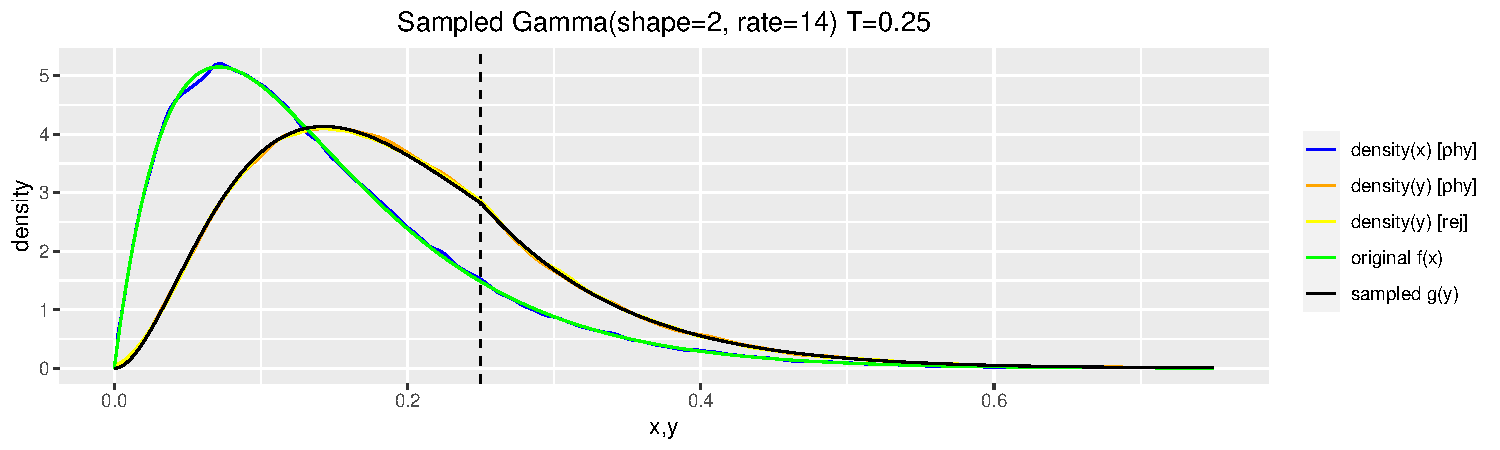
\includegraphics[width=1.0\textwidth]{sampling_event_duration_files/figure-latex/cons_check_nice_colorful-1} \end{center}

The two generators empirical densities for \(y\) lay perfectly over the
sampled theoretical density (shown in black), and the same goes for the
original \(x\) duration draws (the original theoretical density is shown
in green).

Next, consider the Exponential case:

\begin{center}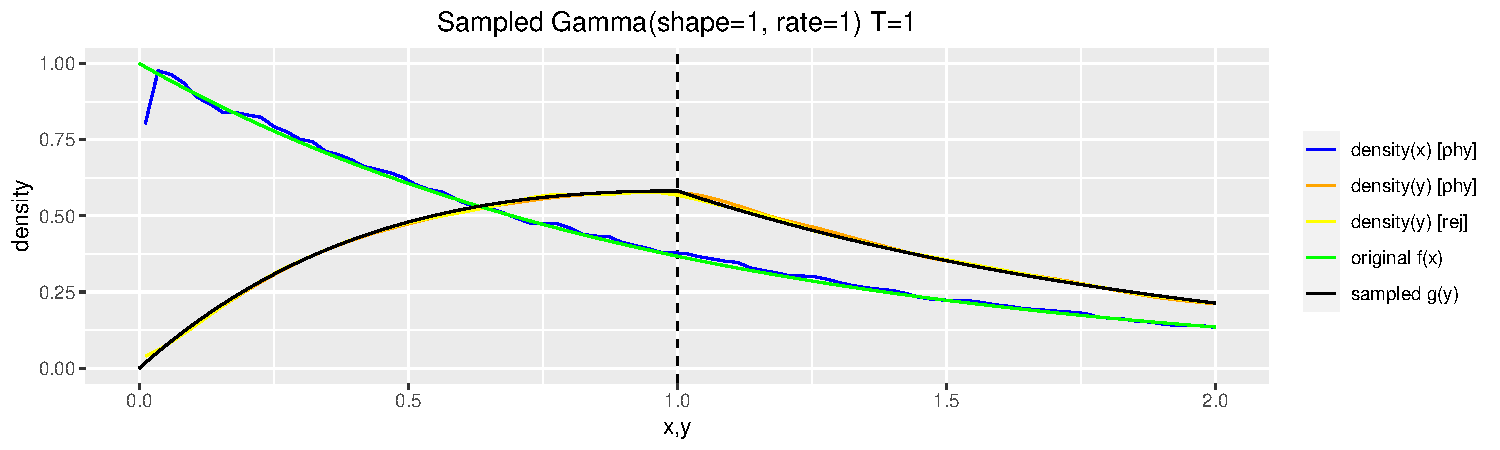
\includegraphics[width=1.0\textwidth]{sampling_event_duration_files/figure-latex/cons_check_arount_t-1} \end{center}

Note the same perfect juxtaposition around T, the critical value around
which the density changes\footnote{also note that the density is still
  continuous at T, but the first derivative is not} its silhouette.

\hypertarget{reparameterization-and-a-look-at-the-likelihood}{%
\section{Reparameterization (and a look at the
Likelihood)}\label{reparameterization-and-a-look-at-the-likelihood}}

The following well-know formulae allows us to reparameterize the Gamma
in term of the expected mean and standard deviation: \[
  x \sim Gamma(\alpha, \beta)   
  \implies
  \begin{cases}
    \mu \triangleq E[x] = \alpha / \beta \\
    \sigma \triangleq sd[x] = \sqrt{\alpha / \beta^2 }
  \end{cases}
  \implies
  \begin{cases}
    \alpha = \mu^2 / \sigma^2 \\
    \beta = \mu   / \sigma^2
  \end{cases}
\] The main motivation for this change of parameters is for Bayesian
analysis, since prior knowledge is usually expressed in term of \(\mu\)
and \(\sigma\) rather than \(\alpha\) and \(\beta\); for example, we may
probably easily know that the a-priori wait time for a storage disk is
5msec \(\pm\) 1 msec from previous measurements or from the disk
technical specification, but it is less likely (in general) that we know
plausible intervals for \(\alpha\) and \(\beta\).

Let's now take a look at the resulting likelihoods shapes, by taking
some draws from a Sampled Gamma and then calculating the log-likelihood
over a grid around the parameter values. Let's consider again the two
densities we used in the ``consistency check'' section:

\begin{center}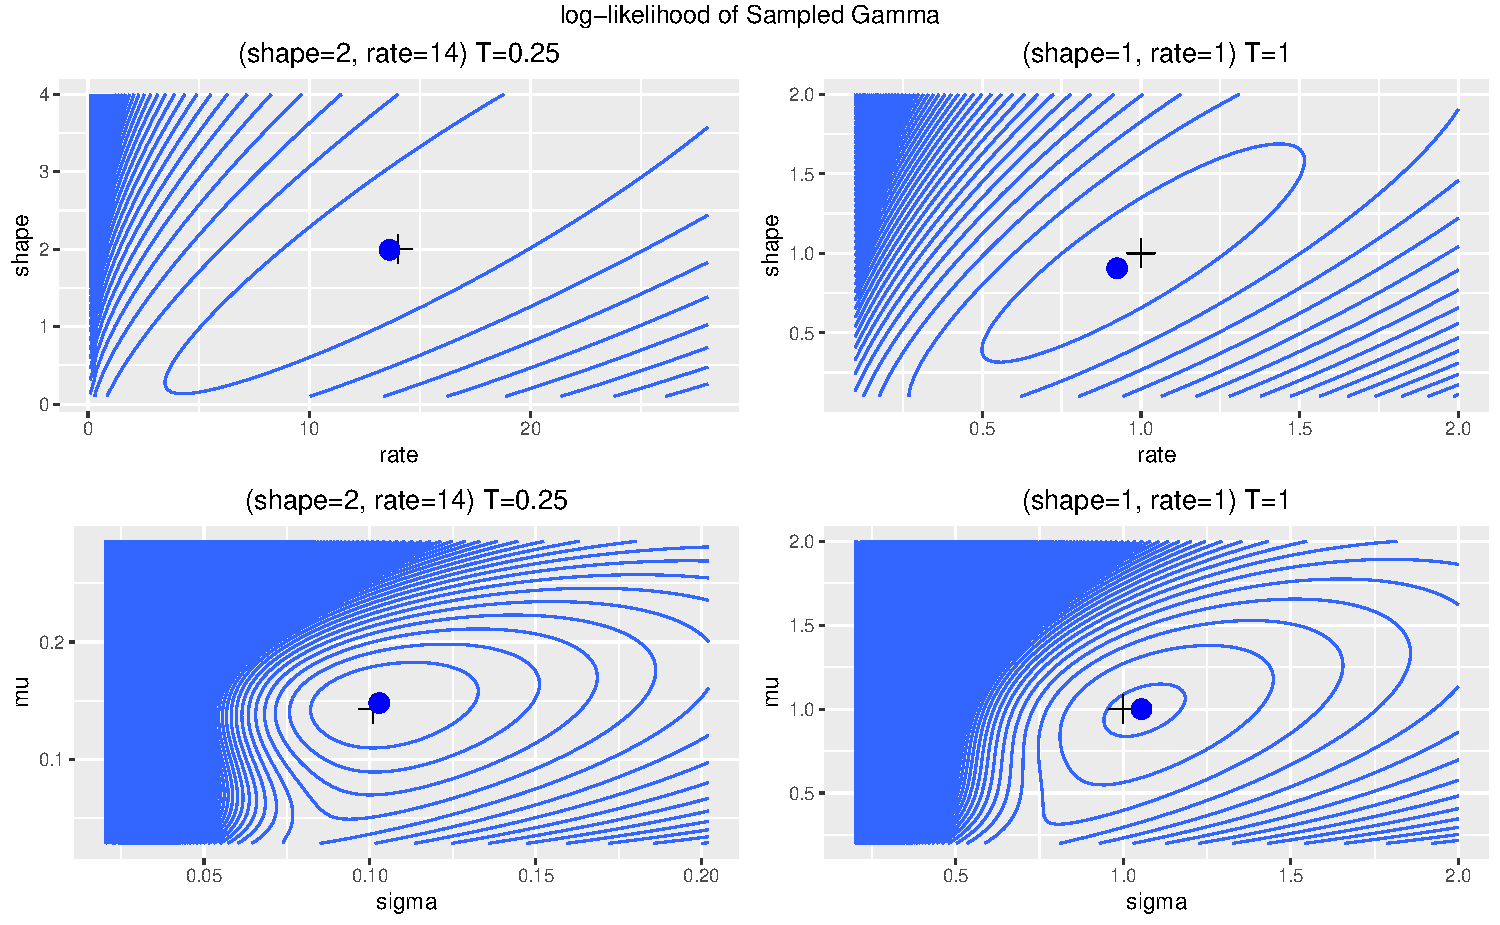
\includegraphics[width=1.0\textwidth]{sampling_event_duration_files/figure-latex/likelihood.explore-1} \end{center}

We can see that the maximum value (the big blue dot) is very close to
the true value (the black cross). Also, the curve looks continuous
(probably concave in general), and that bodes well for using an
algorithm like gradient-descent to build an MLE estimator.

\hypertarget{bayesian-inference-by-stan}{%
\section{Bayesian Inference by Stan}\label{bayesian-inference-by-stan}}

The sampling process, as we have seen, might sample only a small portion
of the original durations (e.g.~one out of 1,000 for durations around
1msec if \(T\)=1sec), and that might leave us with very few data to
build our inference on. Mathematical models are preferable in general
with small datasets, and Bayesian models in particular, since they can
incorporate prior (or ``domain'') knowledge to further improve the
inference.

We will explore the simple case of uninformative priors, both for
simplicity and because the results should be nearly the same we might
obtain using MLE or similar Frequentist techniques. Adding other priors
in the Stan model is definitely trivial anyway.

We will parameterize the model by \(\mu\) and \(\sigma\) mostly because,
as already discussed, prior knowledge is probably more readily expressed
on these parameters rather then on \(shape\) and \(rate\).

Side note: another reason is that the chains seem to converge quicker
using \(\mu\) and \(\sigma\), but I have not made an exhaustive
comparison, so take my word with a grain of salt; yet, the likelihood
plots previously shown seem to indicate a smaller correlation between
\(\mu\) and \(\sigma\) than between \(shape\) and \(rate\).

I have of course checked the chains convergence using the usual
techniques (visual inspection of the chains, Gelman-Rubin statistics,
etc). I will not plot them for the sake of brevity; interested readers
can inspect them by activating the plots in the original Rmarkdown
source\footnote{just knit with stan.inference.print.conv set to TRUE}.

Here's the Stan model:

\begin{Shaded}
\begin{Highlighting}[]
\NormalTok{stan_model_code <-}\StringTok{ "}
\StringTok{functions \{}
\StringTok{  real sampled_gamma_lpdf(data real[] x, real shape, real rate, data real T) \{}
\StringTok{    real T_log = log(T) ;}

\StringTok{    // calc eta}
\StringTok{    real A_log = (-T_log) + }
\StringTok{                 (-log(rate)) + }
\StringTok{                 lgamma(shape+1.0) - lgamma(shape) + gamma_lcdf ( T | (shape+1.0), rate ); }
\StringTok{    real A = exp(A_log) ; }
\StringTok{    real B = 1.0 - gamma_cdf ( T, shape, rate );}
\StringTok{    real eta_log = log(A + B);}
\StringTok{    }
\StringTok{    // calc density}
\StringTok{    real acc = 0.0;}
\StringTok{    for (i in 1:num_elements(x)) \{}
\StringTok{      real xx = x[i];}
\StringTok{      real f_log = gamma_lpdf(xx | shape, rate);}
\StringTok{      real h_log = xx < T ? log(xx) - T_log : 0.0;}
\StringTok{      real d_log = f_log + h_log - eta_log;}
\StringTok{      acc += d_log;}
\StringTok{    \}}
\StringTok{    return acc;}
\StringTok{  \}}

\StringTok{  real sampled_gamma_mu_sigma_lpdf(data real[] x, real mu, real sigma, data real T) \{}
\StringTok{    real shape = mu^2 / sigma^2;}
\StringTok{    real rate  = mu   / sigma^2;}
\StringTok{    return sampled_gamma_lpdf(x | shape, rate, T);}
\StringTok{  \}}
\StringTok{\}}
\StringTok{data \{}
\StringTok{  int<lower=0> N;}
\StringTok{  real y[N]; }
\StringTok{  real T;}
\StringTok{\}}
\StringTok{parameters \{}
\StringTok{  real<lower=0> mu;}
\StringTok{  real<lower=0> sigma;}
\StringTok{\}}
\StringTok{model \{}
\StringTok{  mu    ~ uniform(0.0000001, 100000); // uninformative prior}
\StringTok{  sigma ~ uniform(0.0000001, 100000); // uninformative prior}
\StringTok{  y ~ sampled_gamma_mu_sigma_lpdf(mu, sigma, T);}
\StringTok{\}}
\StringTok{generated quantities \{}
\StringTok{  real shape = mu^2 / sigma^2;}
\StringTok{  real rate  = mu   / sigma^2;}
\StringTok{\}}

\StringTok{"}
\end{Highlighting}
\end{Shaded}

Note that the core of the model is a simple translation (almost a
copy-and-paste) of dsgamma from R to the Stan language\footnote{it is
  also re-parameterized using a simple wrapper function, and by skipping
  the wrapper one can get back the parameterization in term of \(shape\)
  and \(rate\).}. Also note the uninformative priors, and that in the
posterior MCMC samples we derive \(shape\) and \(rate\) as well for
convenience.

Let's now investigate the inference, by generating 100 duration samples,
feeding them to Stan to get back the posterior MCMC chains, and by
plotting both PMDE (Posterior Mean Density Estimate), the density curve
whose parameters are the mean of the posterior chains, and the PSDS
(Posterior Samples Density Set), a smattering of densities whose
parameters are chosen at random from the posterior chains.

Here are the final inferences for our usual pair of densities. First,
consider the generic Gamma:

\begin{center}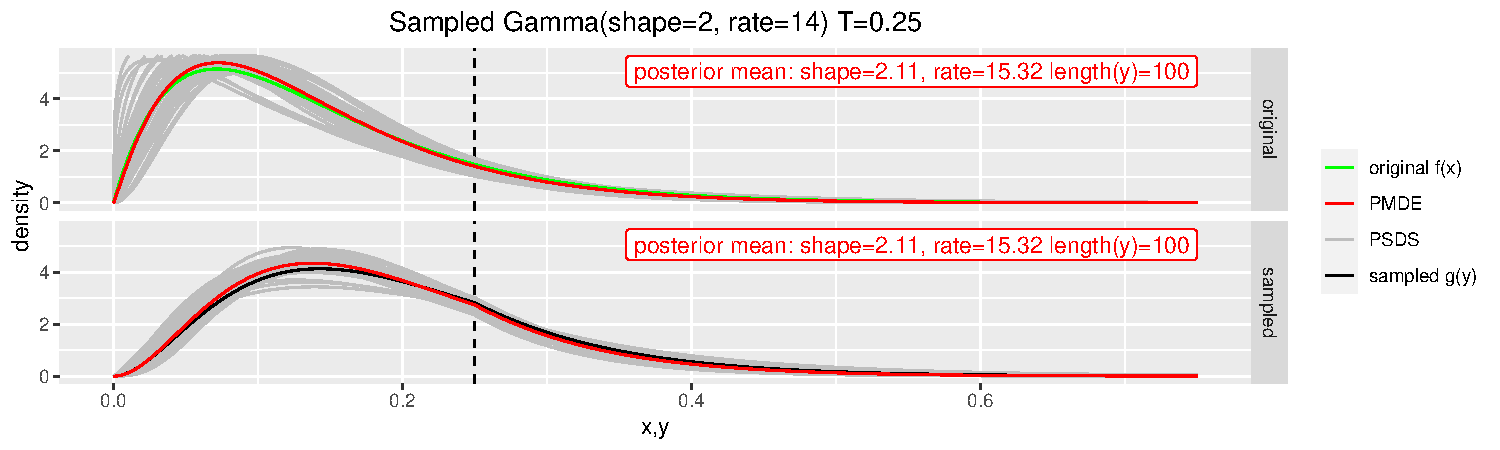
\includegraphics[width=1.0\textwidth]{sampling_event_duration_files/figure-latex/stan_inference_plot1-1} \end{center}

We can see that the PMDE closely fits the true density curve, and that
the PSDS are packed around it, albeit not very tightly, as expected
given the low number of samples.

Next, consider the exponential:

\begin{center}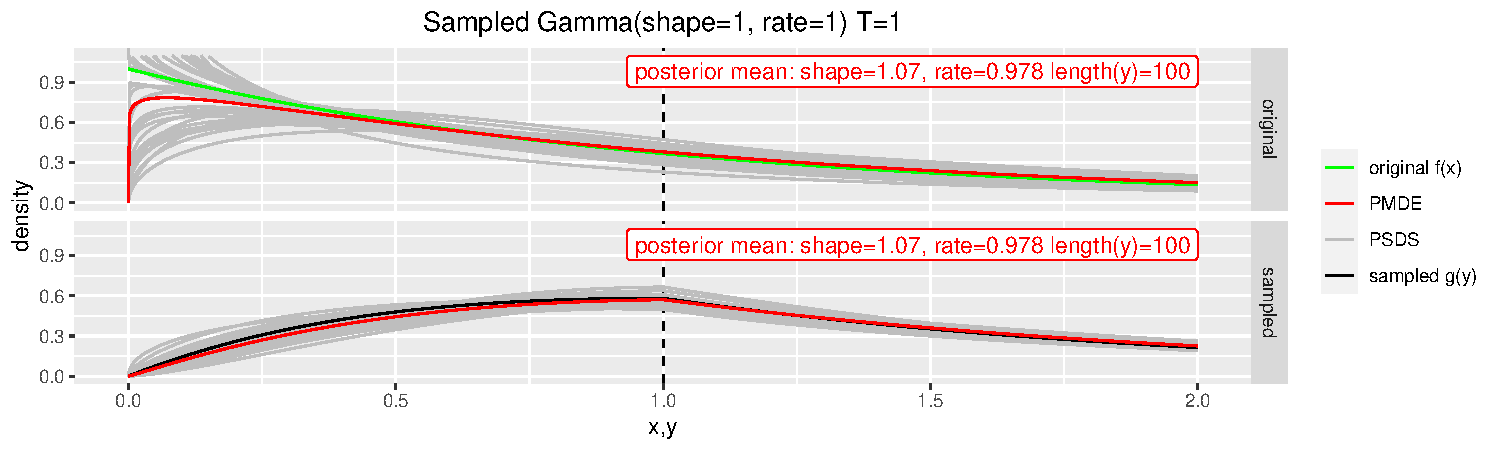
\includegraphics[width=1.0\textwidth]{sampling_event_duration_files/figure-latex/stan_inference_plot2-1} \end{center}

Both the PMDE and the PSDS seem to be qualitatively near to the true
density for \(x\) \textgreater{}\textgreater{} 0, and far from it for
\(x\) near zero. But, this is actually an intrinsic issue for the
exponential distribution when considered as a particular case of the
Gamma: you can never get accurate estimates for \(x\) near to zero. This
is because \[
    \lim_{x \to 0} Gamma(x | \alpha,\beta) = \begin{cases}
      +\infty & \alpha < 1 \\
      \beta & \alpha = 1 \\
      0 & \alpha > 1
    \end{cases}
\]

Hence any error of the \(shape\) estimate will make you drift away from
\(beta\), towards zero or \(+\infty\) depending on the error sign,
whatever small the error modulus is, as patently obvious from the PSDS
plot above.

In other words: the behaviour for \(x\) near zero is
structural\footnote{if there are strong (theoretical?) reasons to
  believe that the true density is actually exponential, the best
  approach is probably to use an exponential model instead of a Gamma
  one. One could simply plug the exponential as \(f(x)\) in the first
  formulae we derived, or could possibly use our Stan model by forcing
  \(shape\) = 1.}, nothing is wrong with the Bayesian estimate.

Of course the estimates neatly improve if more data is available. Here
are the results with a dataset of 1000 duration samples:

\begin{center}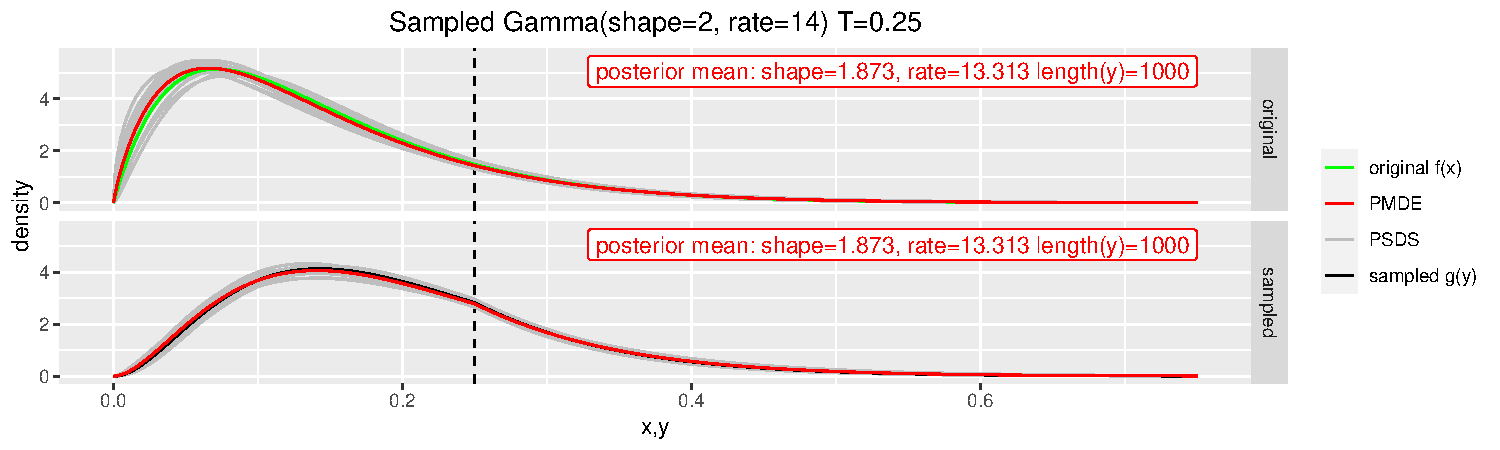
\includegraphics[width=1.0\textwidth]{sampling_event_duration_files/figure-latex/stan_inference_plot1_bis-1} \end{center}

\begin{center}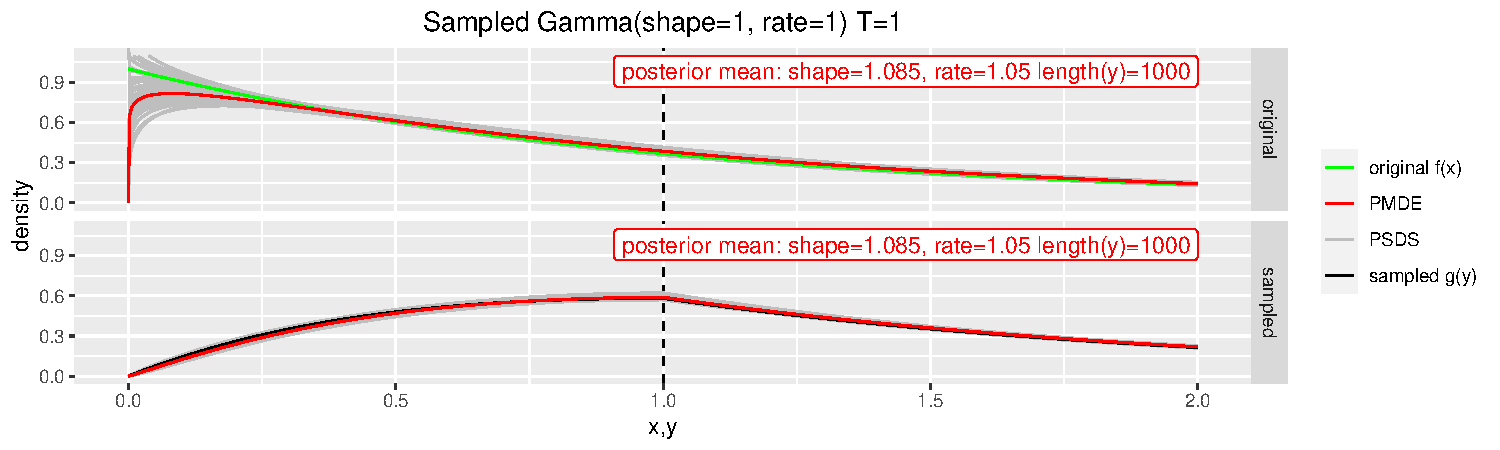
\includegraphics[width=1.0\textwidth]{sampling_event_duration_files/figure-latex/stan_inference_plot2_bis-1} \end{center}

\hypertarget{conclusion-and-next-steps}{%
\section{Conclusion, and next steps}\label{conclusion-and-next-steps}}

We have explored a Bayesian way to infer the parameters of a duration
distribution given some samples over an uniform interval, focusing on
the versatile Gamma distribution. We have simulated the data and the
sampling process using R and the Stan MCMC tool, exploring the fitness
of the estimates to the true data using conventional Bayesian
techniques.

The next obvious step is to experiment with real data. The most
challenging step is to choose a good distribution for the physical
process that we want to study; for software program statistical
profilers (including ASH) we should probably use a distribution arising
from Queueing Theory, since ``everything is a Queue'' inside a computer,
after all.

Using Bayesian Statistics would also allows us to factor in expert
knowledge, that would dictate which Prior to use (I have used only
uninformative priors in the paper, for simplicity). For example, an
expert might tell us that the average disk response time is between
0.5ms and 3msec, and that would certainly help both the precision of the
estimates and the MCMC convergence.

And the ``expert'' might be an automated tool that mined historical
data, producing a general, broad Prior to be used as input.

Document version: 2021/01/09

© 2020-2021 Alberto Dell'Era. Licensed as CC-BY-4.0 License.

\hypertarget{references}{%
\section{References}\label{references}}

Gihub repository:
(\url{https://github.com/alberto-dellera/sampling_event_duration}), with
the Rmarkdown source

\hypertarget{refs}{}
\leavevmode\hypertarget{ref-ASHMATH}{}%
Beresniewicz, John. 2020. \emph{DB Time, Average Active Sessions, and
Ash Math - Oracle Performance Fundamentals}. RMOUG.
\url{https://t.co/wjz3blBIkv?amp=1}.

\leavevmode\hypertarget{ref-DBDA2E}{}%
Kruschke, John K. 2015. \emph{Doing Bayesian Data Analysis: A Tutorial
with R, Jags, and Stan}. 2nd ed. Academic Press / Elsevier.
\url{https://sites.google.com/site/doingbayesiandataanalysis}.

\end{document}
